\title{Excercise 1}
\author{\Large
	\textsc{Markus Korpinen} \\
	\textsc{Teemu Laakso} \\
	\mbox{}\\
	Basics if Monte Carlo -simulations\\
	Department of Physics, University of Helsinki
}
\date{\today}

\documentclass[12pt]{article}

\usepackage{graphicx}
\DeclareGraphicsExtensions{.pdf,.png,.jpg}

\usepackage[utf8]{inputenc}
\usepackage[T1]{fontenc}
\usepackage[paper=a4paper,dvips,top=2.5cm,left=2.5cm,right=2.5cm,
    foot=1cm,bottom=4cm]{geometry}
\usepackage[fleqn]{amsmath}

% Various AMS fonts.
\usepackage{amsfonts}

% Many special mathematical characters, including the
% famous blackboard bold letters used.
\usepackage{amssymb}

% Theorems using the AMS style.
\usepackage{amsthm}
% The following is probably the optimal method for numbering
% lemmas, examples, definitions their like. We number them
% all together. It is annoying and difficult
% for the reader to search for these theorem-like entities in
% if they are.

\renewcommand{\textfraction}{0.01}
% Numbering of theorems is by section, e.g., Theorem 1.3, etc.
% This makes it easier for the reader to search for them.

\newtheorem{theorem}{Theorem}[section]
\newtheorem{definition}[theorem]{Definition}
\newtheorem{lemma}[theorem]{Lemma}
\newtheorem{corollary}[theorem]{Corollary}
\newtheorem{fact}[theorem]{Fact}
\newtheorem{example}[theorem]{Example}

% If the paper has a large number of equations, figures, tables, etc.,
% then they should be numbered within sections. Comment out
% if this is not what you want.
\numberwithin{equation}{section}
%\numberwithin{figure}{section}
\numberwithin{table}{section}


%\usepackage{showkeys}

\begin{document}


\maketitle

\newpage{}

%\tableofcontents{}

\section*{Problem 1}

\begin{equation*}
P_{hit}=P_1*P_2,
\end{equation*}
where $P_1$ is the probability that center of needle is less than $l/2$ away from line and $P_2$ is the the probability that the needle is in a right angle to cross the line. Probabilities $P_1$ and $P_2$ are depending on each other so they have to be multiplied. Because $P_1$ can fall to eather side of line 
\begin{equation*}
P_1=\frac{l/2+l/2}{d}=\frac{l}{d}.
\end{equation*}
Probability that needle crosses the line when center falls x away is a function of x. The probability $P_2$ when needle drops somewhere can be obtained by integrating and setting $l=2$ (unit circle)
\begin{equation*}
P_2=4\int_{0}^{1}\frac{cos^{-1}(x)}{2\pi}dx=\frac{2}{\pi}.
\end{equation*}
Therefore
\begin{equation*}
P_{hit}=P_1*P_2=\frac{2l}{\pi d}.
\end{equation*}
\subsection*{a)}
\begin{figure}[H]
	\caption{When you throw only 10 times the predicted value for $\pi$ is bad.}
	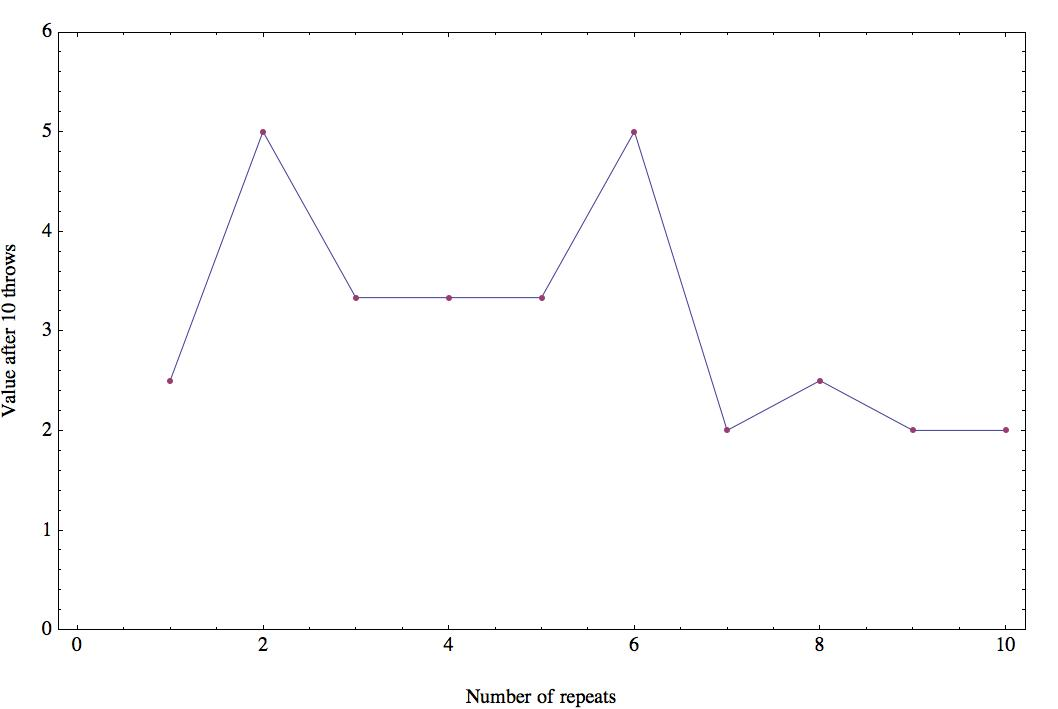
\includegraphics[width=15cm]{mc_p01_a.jpg}
\end{figure}
\subsection*{a)}
\begin{figure}
\caption{After approximately 5000 throws result starts to converge.}
	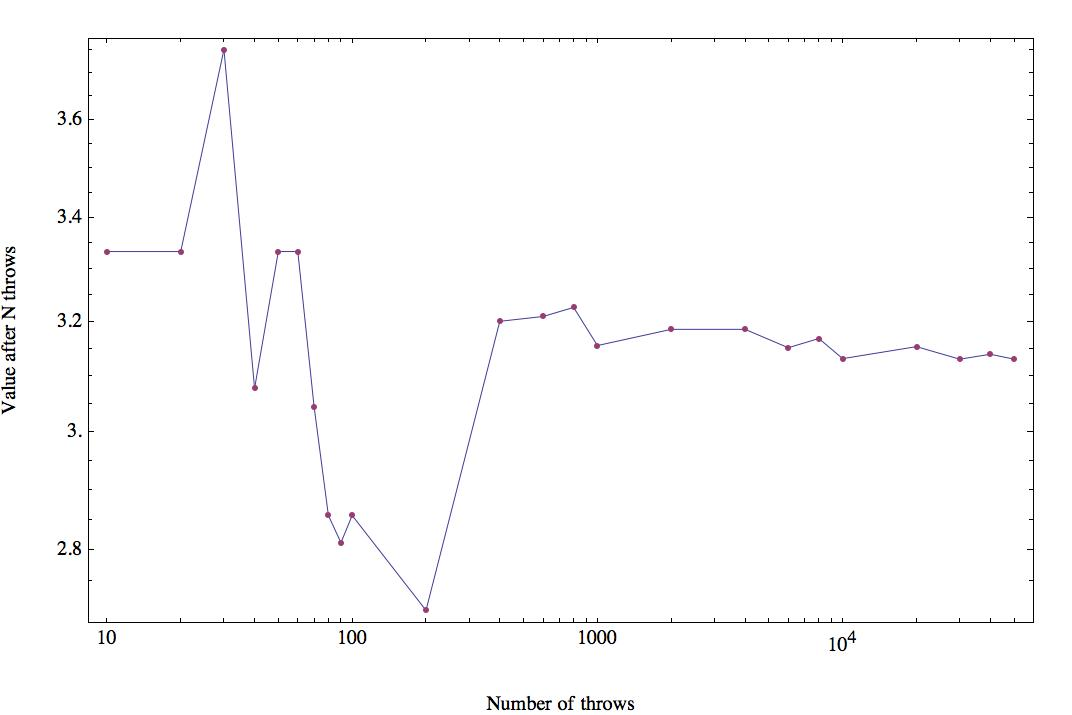
\includegraphics[width=15cm]{mc_p01_b.jpg}
\end{figure}

\section*{Problem 3}
\begin{figure}
\caption{100 numbers generated with the quick-and-dirty generator}
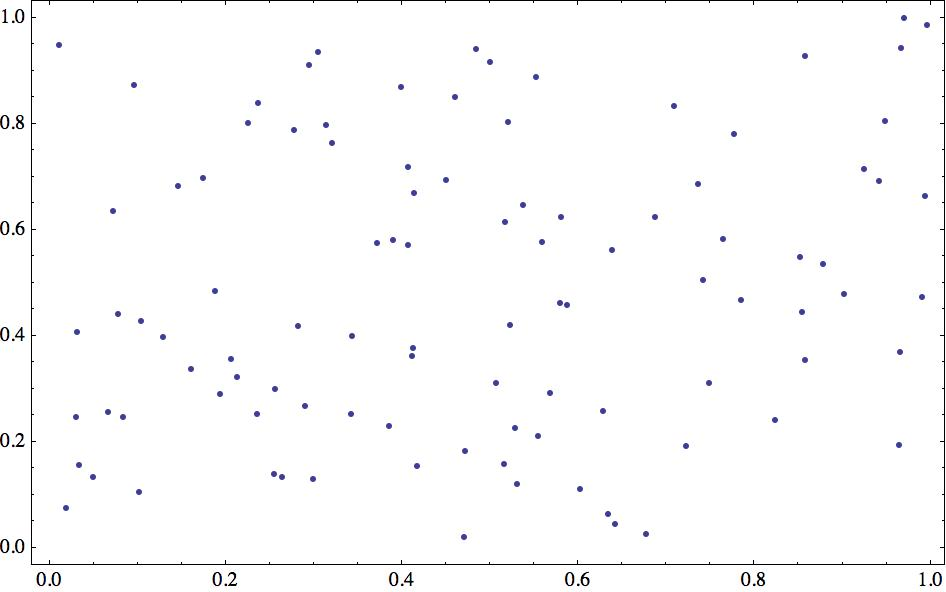
\includegraphics[width=15cm]{qd1.jpg}
\end{figure}
\begin{figure}
\caption{10000 numbers generated with the quick-and-dirty generator}
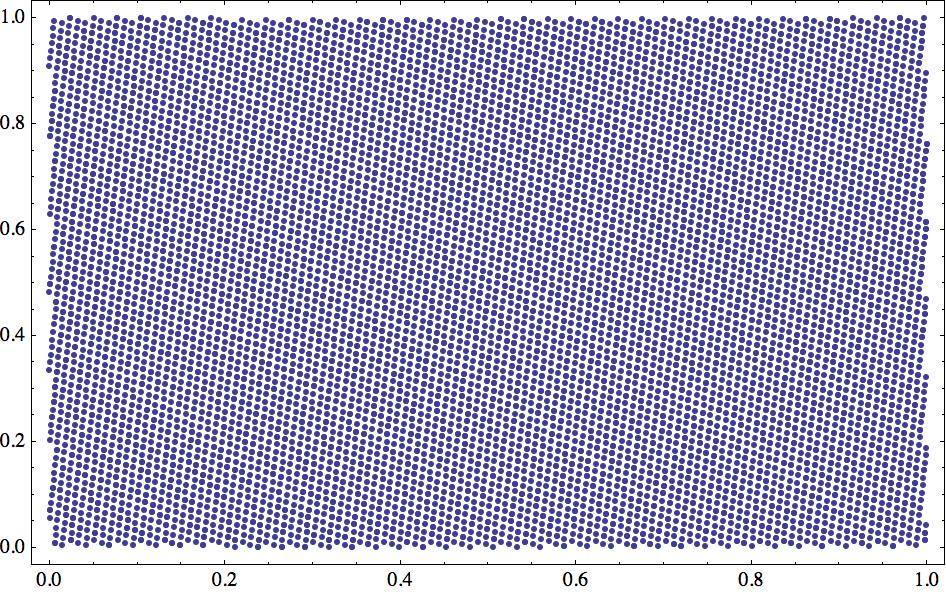
\includegraphics[width=15cm]{qd2.jpg}
\end{figure}
\begin{figure}
\caption{100 numbers generated with the Park-Miller generator}
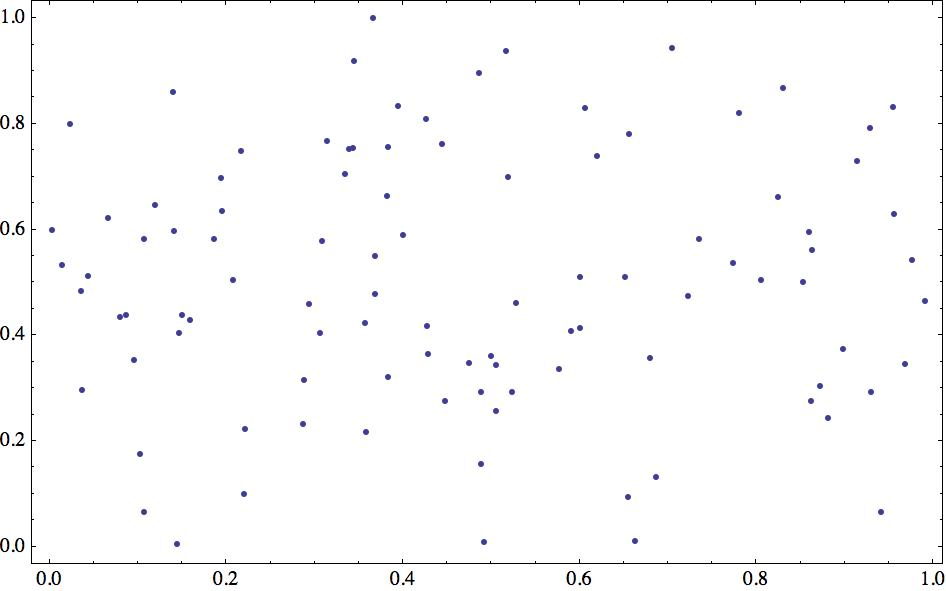
\includegraphics[width=15cm]{pm1.jpg}
\end{figure}
\begin{figure}
\caption{10000 numbers generated with the Park-Miller generator}
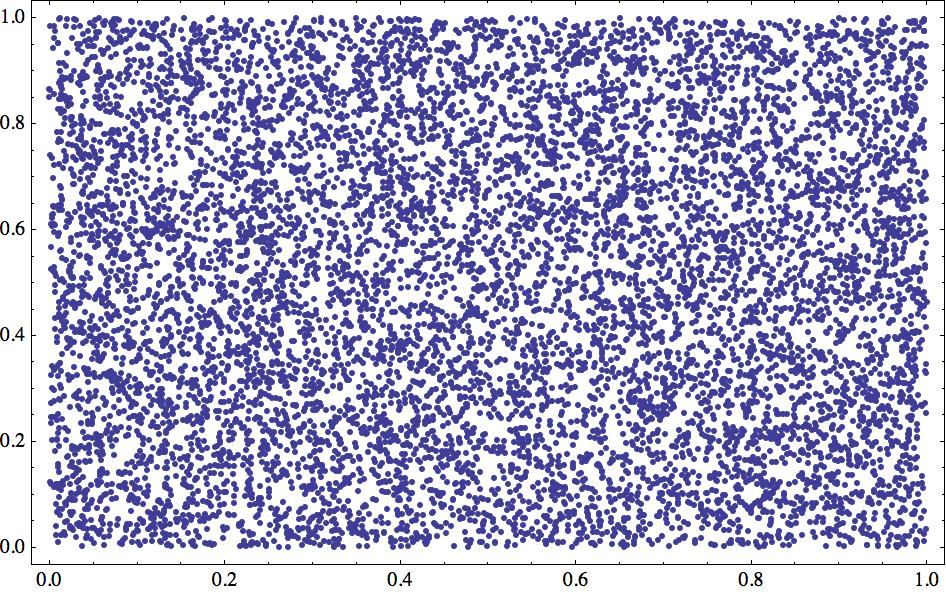
\includegraphics[width=15cm]{pm2.jpg}
\end{figure}

\section*{Problem 4}
\begin{figure}
\caption{10 000 points with the quick-and-dirty generator with interval x=[0, 0.0001]}
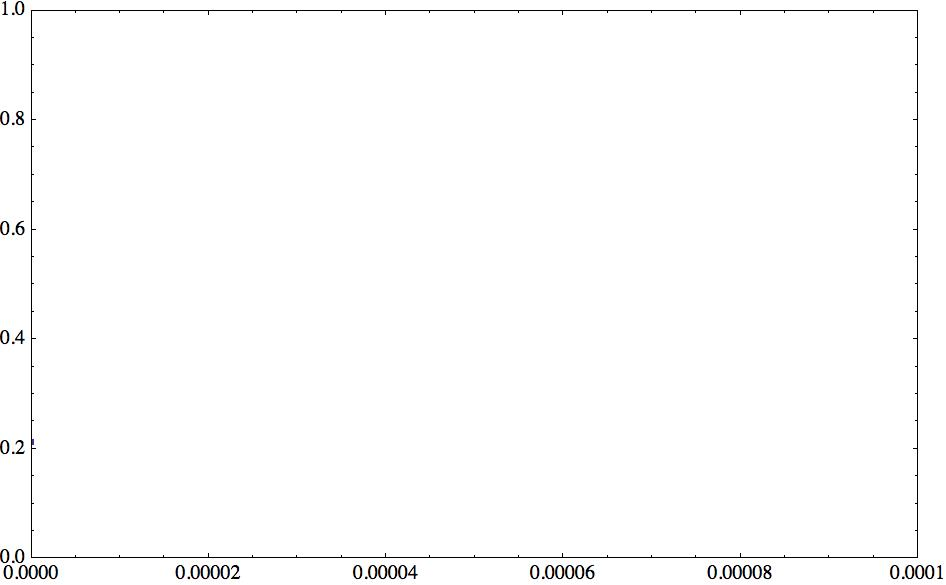
\includegraphics[width=15cm]{qd3.jpg}
\end{figure}
\begin{figure}
\caption{10 000 points with the quick-and-dirty generator with interval x=[0, 0.001]}
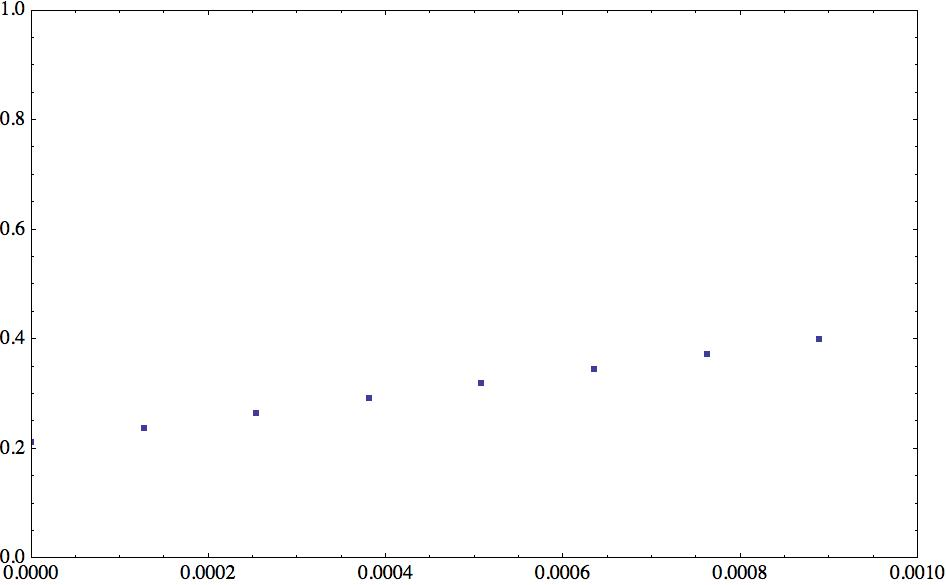
\includegraphics[width=15cm]{qd4.jpg}
\end{figure}
\begin{figure}
\caption{10 000 points with the Park-Miller generator with interval x=[0, 0.0001]}
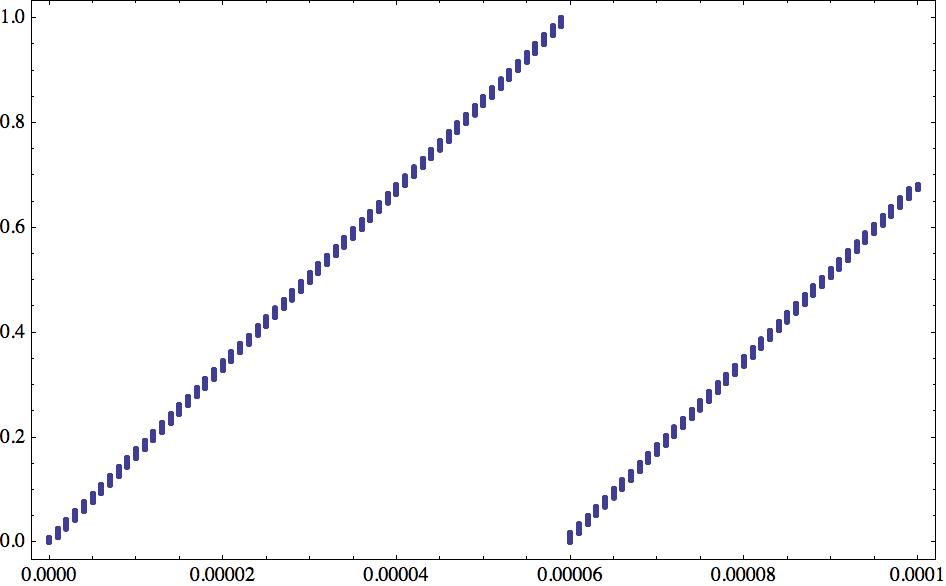
\includegraphics[width=15cm]{pm3.jpg}
\end{figure}
\begin{figure}
\caption{10 000 points with the Park-Miller generator with interval x=[0, 0.001]}
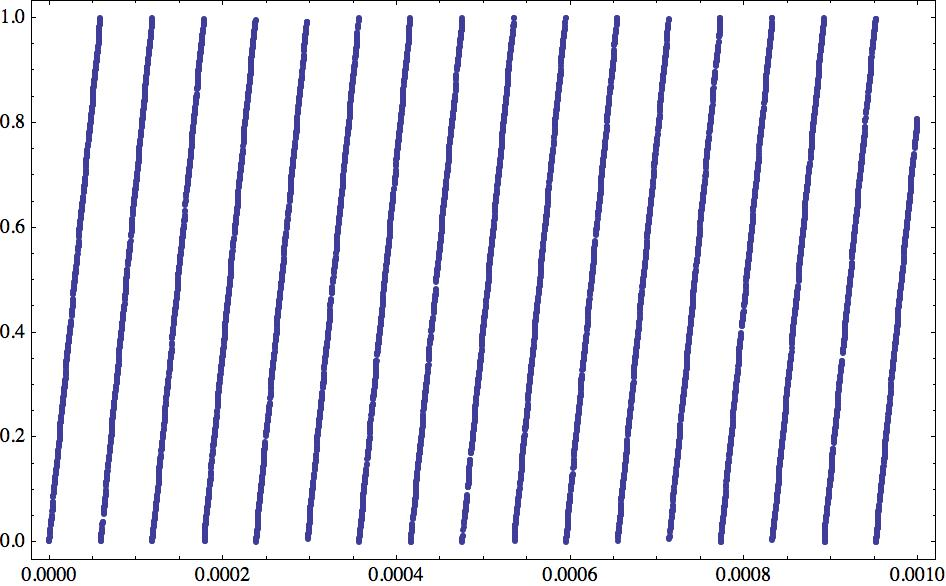
\includegraphics[width=15cm]{pm4.jpg}
\end{figure}



\section*{Problem 6}
Following block of code can be found from the source code of Mersenne Twister:

\begin{tabbing}
\texttt{/* initializes mt[N] with a seed */}\\
\texttt{void init\_genrand( unsigned long s) }\\
\texttt{\{} \ \= \+ \\
\texttt{ mt[0]= s \& 0xffffffffUL;}  \\
\texttt{    for}\=\texttt{ (mti=1; mti<N; mti++) \{ }\+\\
\texttt{        mt[mti] = }\\
\texttt{	    (1812433253UL * (mt[mti-1] \^ (mt[mti-1] >> 30)) + mti); }\\
\texttt{        /* See Knuth TAOCP Vol2. 3rd Ed. P.106 for multiplier.}\\ %*/
\texttt{       /* In the previous versions, MSBs of the seed affect  */}\\
\texttt{        /* only MSBs of the array mt[].                        */}\\
\texttt{        /* 2002/01/09 modified by Makoto Matsumoto            }\\ %*/
\texttt{       mt[mti] \&= 0xffffffffUL;}\\
\- \texttt{       /* for >32 bit machines */}\\
\- \texttt{    \}}\\
\texttt{\}}
\end{tabbing}
\end{document}